\documentclass[tikz]{standalone}
\usepackage{pgfplots}
\pgfplotsset{compat=1.15}
\usepackage{mathrsfs}
\usetikzlibrary{arrows,calc}
\usepackage{tkz-euclide}
\pagestyle{empty}

\definecolor{AngleClr}{rgb}{0,0.39215686274509803,0}
\definecolor{ShapeClr}{rgb}{0.6,0.2,0}

\definecolor{BlueClr}{RGB}{71, 113, 158}
\definecolor{GreenClr}{RGB}{129, 196, 120}
\definecolor{RedClr}{RGB}{204, 98, 59}

\begin{document}

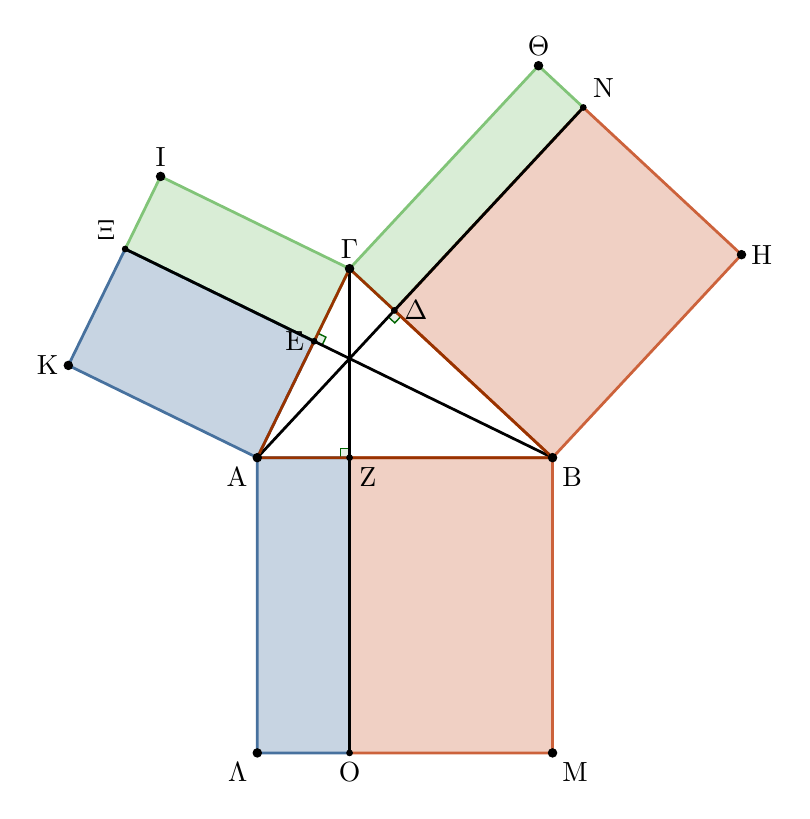
\begin{tikzpicture}[scale=.75]
\tkzSetUpLine[line width=1pt,color=black]
\tkzSetUpPoint[fill=black]

\tkzDefPoints{0/0/A,5/0/B,1.5625/3.2/C}

\tkzFillPolygon[fill=white](A,B,C)

\tkzDefSquare(C,B) \tkzGetFirstPoint{H} \tkzGetSecondPoint{Th}
\tkzDefSquare(A,C) \tkzGetFirstPoint{I} \tkzGetSecondPoint{K}
\tkzDefSquare(B,A) \tkzGetFirstPoint{L} \tkzGetSecondPoint{M}

\tkzDefPointBy[projection=onto H--Th](A)\tkzGetPoint{N}
\tkzDefPointBy[projection=onto I--K](B)\tkzGetPoint{Xi}
\tkzDefPointBy[projection=onto L--M](C)\tkzGetPoint{O}

\tkzInterLL(A,N)(B,C) \tkzGetPoint{D}
\tkzInterLL(B,Xi)(A,C) \tkzGetPoint{E}
\tkzInterLL(C,O)(A,B) \tkzGetPoint{Z}

\tkzFillPolygon[fill=GreenClr,draw=GreenClr,fill opacity=0.3,line width=1pt](C,D,N,Th)
\tkzFillPolygon[fill=GreenClr,draw=GreenClr,fill opacity=0.3,line width=1pt](C,E,Xi,I)

\tkzFillPolygon[fill=RedClr,draw=RedClr,fill opacity=0.3,line width=1pt](B,H,N,D)
\tkzFillPolygon[fill=RedClr,draw=RedClr,fill opacity=0.3,line width=1pt](B,Z,O,M)

\tkzFillPolygon[fill=BlueClr,draw=BlueClr,fill opacity=0.3,line width=1pt](A,Z,O,L)
\tkzFillPolygon[fill=BlueClr,draw=BlueClr,fill opacity=0.3,line width=1pt](A,E,Xi,K)
% \tkzFillPolygon[fill=green](A,C,H,Th)

\tkzMarkRightAngles[line width=0.5pt, size=.15,color=AngleClr,fill=AngleClr,fill opacity=0.1](C,Z,A B,E,C A,D,B)

% \tkzDrawSegments[line width=0.5pt,color=black,dashed,dash pattern=on 1pt off 1.75pt](B,H B1,H C,C1 A,B2 B2,B1 C2,A2)
% \tkzDrawSegments[line width=0.5pt,color=black,dashed,dash pattern=on 1pt off 1.75pt,add=0 and 0.3](A,H)

\tkzDrawSegments[line width=1pt,color=black](C,O B,Xi A,N)

\tkzDrawPolygon[color=ShapeClr](A,B,C)
\tkzDrawPoints[size=3](A,B,C)
\tkzDrawPoints[size=2](D,E,Z)
\tkzDrawPoints[size=3](H,Th,I,K,L,M)
\tkzDrawPoints[size=2](N,Xi,O)
\tkzLabelPoint[below left](A){$\rm A$}
\tkzLabelPoint[below right](B){$\rm B$}
\tkzLabelPoint[above](C){$\rm \Gamma$}
\tkzLabelPoint[right](D){$\rm \Delta$}
\tkzLabelPoint[left](E){$\rm E$}
\tkzLabelPoint[below right](Z){$\rm Z$}

\tkzLabelPoint[right](H){$\rm H$}
\tkzLabelPoint[above](Th){$\rm \Theta$}
\tkzLabelPoint[above](I){$\rm I$}
\tkzLabelPoint[left](K){$\rm K$}
\tkzLabelPoint[below left](L){$\rm \Lambda$}
\tkzLabelPoint[below right](M){$\rm M$}

\tkzLabelPoint[above right](N){$\rm N$}
\tkzLabelPoint[above left](Xi){$\rm \Xi$}
\tkzLabelPoint[below](O){$\rm O$}

% \tkzMarkSegments[mark=s||,size=2.5](O,A O,B O,C)

\end{tikzpicture}

\end{document}
